\chapter{Signals and Lanes \who{Grether, Thunig}}
\label{ch:signalslanes}
% ##################################################################################################################

\hfill \textbf{Author:} Dominik Grether, Theresa Thunig

\begin{center} 
\includegraphics[width=0.25\textwidth, angle=0]{figures/MATSimBook.png} \end{center}

% ##################################################################################################################

\section{Motivation}

%\mnote{Traffic Signal Control}
Traffic signals ensure security of travelers at junctions and regulate right of way. 
Furthermore, by assigning green times to the different approaches of a junction they are a determinant of the junctions performance. 
There are different strategies for traffic signal control: fixed-time traffic signal control for example repeats periodically the same schedule for signalization, whereas traffic-responsive signal control reacts dynamically on the prevailing traffic patterns to improve the performance of the junction or the system as a whole.   
Even if traffic %-responsive 
control improves the traffic conditions at a single junction, it might not result in benefits for the system as a whole. 
% As result of an improved traffic-responsive signal control at two single junctions, network wide changes in travel patterns can evolve}~\cite{Burghout2007HybridSimulationAdaptiveSignal}. 
\citet{Hu1997D2DFlowEvolutionReactiveSignalsDynasmart} argue that
second order or network effects should be taken into account when effects of signal control strategies are tested. Network effects include drivers' reactions not only in terms of route choice but also in terms of scheduling. 
Thus, traffic control and especially traffic-responsive signals need to obey some constraints. Otherwise, traffic may become unstable at the network level. 
%Thus, traffic-responsive signals can perform much worse than a fixed-time control in some situations~\citep{LaemmerHelbing2010SelfStabilizingSignalControlRealNet}. 
MATSim can capture most of these effects. 

This chapter reviews concepts, usage, and restrictions of the traffic signal control extension for MATSim. 
Before we will go into details, to motivate traffic signal with MATSim, a case study is reviewed. 
%TODO dg refer to time dependent network alternative, see diss and charypar thesis
%mnote{Traffic Signal Control}
%Traffic signals impose time variant attributes to a transport network. 
%The approaches presented in the first sections of this chapter may be used for modeling. 
%If traffic signals are controlled by a fixed-time control, the problem is periodical. 
%A cyclical time expansion of the network can be applied~\citep{KoehlerStrehler2010SignalDemandOptimization}. 
%However, for large-scale applications memory consumption of time expansion and the resulting network size still limits analysis to subnetworks, see Sec.~\ref{sec:optimized_fixed_time_control}. 
%
%In case of a traffic-responsive signal control, a periodic formulation is no longer suitable.  
%The approach by~\citet{GeorgeShekhar2008TimeAggregatedGraphs} requires too much memory.  
%Instead, the time dependent attributes developed for evacuation scenarios might be considered. 
%For traffic-responsive signal control, the number of changes is clearly higher than for evacuation scenarios. 
%The number of changes, $C$, to the network should be small.
%Otherwise, lookup costs increase logarithmically and memory consumption increases linear in $C$. 
%In case of a traffic-responsive signal control a preprocessing of changes is not feasible. 
%Then, the time dependent attributes have additional, permanent reorganization costs for the binary search tree data structure. 
%Thus, in the following, potential extensions of the traffic flow model of the mobility simulation are considered.

\subsection{Case Study}

The Cottbus scenario presented in Chapter~\ref{ch:scenarios:cottbus} is applied to illustrate the influence of traffic signal control. 
This section summarizes results published in~\citet{GretherBischoffNagel2011CottbusSylviaEventAbstract,Grether2014PhD}, readers interested in details are referred to these publications. 

%
The runs sequence of the base case is performed with three different signal control strategies:
%
In a first simulation sequence, all traffic signals are switched off. This can be used as a lower bound for results concerning signal control since it assumes that vehicles are able to traverse a crossing without any accident, i.e., they are able to drive ``through each other''. 
%
The next sequence uses the fixed-time setup. 
%
In the third, final, sequence, all traffic signals are controlled by a traffic-actuated stage length control. 
The control is based on the pretimed fixed-time schedules. 
The green times of the fixed-time schedules are reduced to a minimal green time of $5$/$10$ $sec.$. 
If at the end of this reduced green time vehicles are still approaching the green time is extended up to a predefined maximum. 

\createfigure%
{Simulation Results}%
{Simulation Results}%
{\label{fig:results_histogram}}
{%
  \createsubfigure%
  {No vs.~fixed-time vs.~traffic-actuated signal control, commuter traffic, iteration 1000}%
	{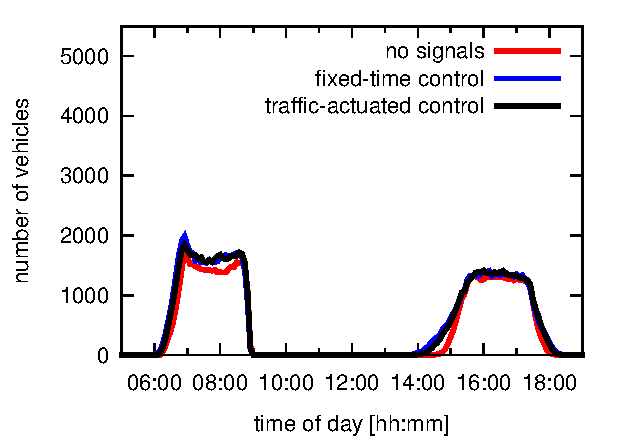
\includegraphics[width=0.48\linewidth]{extending/figures/signalslanes/leg_histogram_1292_1293_1291_it_1000.pdf}}
  {\label{fig:commuter_traffic}}%
  \createsubfigure%
	{Average travel time for unexpected event traffic, iteration 1000}
	{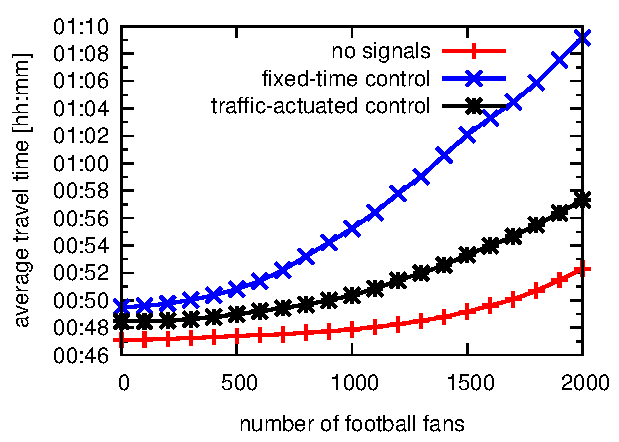
\includegraphics[width=0.48\linewidth]{extending/figures/signalslanes/average_travel_time_1220_1222.pdf}}
	{\label{fig:unexpected_event}}
}%
{Source:~\citet{Grether2014PhD}}

Simulation results for iteration 1000 of the Cottbus commuter scenario are depicted in
Fig.~\ref{fig:commuter_traffic}. 
The number of vehicles simultaneousely on the road is plotted over the time-of-day. 
%Due to the nature of a commuter scenario characterized by a steady
%demand over a certain time horizon 
The results are quite similar for all signal control strategies. 
The differences are small because of the lack of heavy congestion in the Cottbus scenario. 

A change of signal control has more effect if some unexpected traffic occurs in the network. 
It is assumed that the local soccer club ``FC Energie Cottbus'' has a derby that takes place on a normal weekday, thus interfering with the regular commuter traffic. 
In the last iteration of the run sequences, in addition to the commuters $0$ to $2000$ vehicles drive to the soccer stadium of Cottbus during the evening peak. 
It is assumed that 25 \% of these fans come from Cottbus,
while the other 75 \% come from the ``Spree-Nei{\ss}e'' area around Cottbus, and that all fans start their trips between 17:00 and 18:00. 

Fig.~\ref{fig:unexpected_event} plots the number of soccer fans on
the x-axis, and the average travel time of all travelers on the
y-axis. Without any additional vehicles,
the traffic-actuated signal control leads to a gain of
approx.~$1 \, min$ per traveler.
The more additional traffic is approaching the stadium, the more the traffic-actuated control saves travel time. In the case where 2000 additional vehicles are on the road, travel time savings reach ca.~$15\, min$~per traveler. 

Summarizing: In slightly jammed commuter scenarios, simulation results with a change in traffic signal control that leads to heavily decreased overall travel time have not been simulated with MATSim, yet. 
Looking at different objectives with more fine grained analysis tools can reveal network wide effects~\citep[e.g.~see the analysis using macroscopic fundamental diagrams, pp.114]{Grether2014PhD}, but this is work in progress.  
More heavily jammed scenarios can increase the overall traffic impact of a change in traffic signal control. The case study show significant effects of traffic-responsive signal control, if something unexpected happens and travelers do not react.  

\subsection{Overview -- MATSim \& Traffic Signals?}

The presented case study highlights some already researched aspects of MATSim simulations with traffic signals. 
MATSim is not the tool of choice for all questions concerning traffic signal control. 
The codebase, however, can also help to simulate other use cases, e.g.~evacuation or air transport scenarios. 
MATSim's open source nature provides hooks and interfaces for extension. 
But you should consider the amount of work required to get things done in respect to the current state of development and your project planning. 
The remaining chapter provides deeper insight.  
%If you need highly detailed traffic flow models or a high detail network representation, you should consider other tools. 
Sec.~\ref{sec:signals_traffic_signal_control} provides some traffic signal control backgrounds, vocabulary, and options for modeling with MATSim.  
Sec.~\ref{sec:signals_network_traffic_flow} goes into details of network and traffic flow modelling. 
If your requirements are met, Sec.~\ref{sec:signals_iterations_learning} considers iterations and learning. 
When it comes to agent based learning, MATSim is very fast -- the presented case study requires on average~$17$ seconds computation time per iteration -- for scoring, replanning, and output. One complete run sequence ($1000$ iterations, single core mobility simulation, multi core replanning) was simulated in $9 \, h$ and $12 \, min$. 
The speed of simulation leaves room for exploration of network wide behavioral reactions on changes of traffic signal control. 
Furthermore, the resource efficient simulation enables the joint simulation of several policies. 
Before you present your results to public, you should consider certain aspects concerning the  evaluation and interpretation of simulation results. 
Hints are provided in conjunction with a conclusion in Sec.~\ref{sec:signals_evaluation_conclusion}. 
In Sec.~\ref{sec:signals_config} the most important configuration parameters are provided. 
More details can be found in the traffic signals user guide. 
%Thus, it is well worth to consider a extension for the simulation of traffic-responsive signal control. Further, the impacts of recently developed optimization models for fixed-time control can be tested~\citep{KoehlerStrehler2010SignalDemandOptimization}. 


\section{Traffic Signal Control}
\label{sec:signals_traffic_signal_control}

On a coarse level, control strategies for traffic signals can be classified in fixed-time and traffic-responsive strategies. 

Fixed-time traffic signal control periodically assigns green times for each approach of a junction. 
Cycle time and green split are not modified within short periods of time. 
To establish green waves between adjacent junctions the start of green light for the approaches within the cycle can be adjusted in respect to a global timer. 
These shifts are referred as coordination offsets. 
For optimization of fixed-time signals different regimes of equilibrium traffic flow are determined for several periods of time, e.g., weekday morning, midday, evening and night plus a separate estimate for weekends.   
Optimization may target all parameters of a signalized junction -- green split, cycle, offsets, and phase composition. 
%These traffic flows serve as input for optimization~\citep[e.g.~][]{Webster1961SignalSettings,Allsop1972SignalizedJunctionCapacity,Allsop1991SignalsStageBased,Robertson1969Transyt}.  
But, there is no possibility to react on acute changes of equilibrium traffic flows. 

Traffic-responsive control reacts on acute traffic patterns adjusting traffic signal control parameters on the fly. 
In principle all available information on prevailing traffic patterns can be used. 
The diversity of traffic-responsive control algorithms is wide, for a review of some of the reader is referred to~\citet[][]{Grether2014PhD}. 

MATSim's traffic signal module is designed to simulate all different kinds of traffic signal control strategies. 
The module provides a default implementation for fixed-time control. 
Traffic-responsive strategies require custom implementation of the control algorithm but can make use of the existing data formats. 
Data is divided into five different types of input:
\begin{description}
	\item[Signals:] The location of the traffic signal hardware on the network is typically independent from the control strategy. Signals can be located at the end of a link or a lane, see the next section for further discussion of lanes. Signals are attached to a system that reflects e.g.~all signals of a junction or even larger units. Each signal system is controlled by exactly one control algorithm at a time.  
	\item[Signal Groups:] Traffic signals have to be attached to a group. A group of signals shows the same color at the same time. Each time a signal group changes its state a MATSim event is triggered. 
		There is no explicit representation of phases. If required this can be realized on top of the signal groups.  
	\item[Control:] Comprises information for fixed-time control and can be used to specify custom control algorithms per system. 
	\item[Amber:] Specifies the time of amber at the beginning and end of green time. At time of writing this information is only used for visualization purposes. 
		Driving is not permitted if a traffic signal shows amber light. 
	\item[Intergreens:] Specifies the minimal time period between the ending of the one and the beginning of another signal group's green time.  
		This information is fairly important as MATSim's traffic flow model does not contain any collision detection. 
		When available a validation module reads the event stream and triggers a warning or an error if security constraints are violated. 
		Further, customized control strategies can access this information to ensure the validity of control in respect to security aspects.    
\end{description}

The next section considers network representation and location of traffic signals in more detail. 

%\mnote{Traffic-Actuated Control}
%With upcoming availability of sensors and computer technology these optimizations provided the basis for traffic-actuated signal control strategies. 
%Some actuated approaches use logical operators and functions to adjust signal timings~\citep{Friedrich2002VerkehrsadaptiveLSASteuerung}. More advanced methods as, e.g., SCOOT~\citep{HuntEtc1981SCOOT,RobertsonBretherton1991ScootMethod,BrethertonBodgerBaber2004ScootFuture}, MOTION~\citep{BielefeldtBusch1994MOTION,BuschKruse2001MotionSITRAFFIC,BrilonEtAl2009MotionMuenster}, or BALANCE~\citep{GEVAS2011Balance,BraunEtAl2009TravolutionLSA2CarCommunication} use macro- and mesoscopic traffic models to predict effects of adjustments of signal timings for a certain time horizon.  
%%
%
%%\mnote{Adaptive Control}
%Recent approaches for traffic signal control no longer need a fixed-time control that is adjusted. 
%Instead, the signal program is build completely on-the-fly based on sensor information.  
%%
%These methods originate from different areas of science. 
%One finds rather conceptual studies and methods that can and are used in practice. 
%%TUC
%An example for the latter is TUC (traffic-responsive urban control)~\citep{DiakakiPapageorgiouAboudolas2002MultivariableRegulatorTUC,DiakakiEtAl2003ExtensionsTUC,KrausEtAl2010CostEffectiveSignalsTUC,AboudolasEtAl2010RollingHorizonTUC,KouvelasEtAl2011HybridStrategyTUC} a control theoretic strategy that uses a linear-quadratic regulator approach to control green splits based on a store-and-forward model of urban traffic. 
%Due its polynomial complexity TUC can be used in real time monitoring the whole transport network. 
%Optional extensions to TUC provide cycle time adjustments, offset optimization, and public transit priority.   
%Also practice ready is the approach proposed by~\citet{Laemmer2007PhD,LaemmerHelbing2008SelfControlTrafficLights,LaemmerHelbing2010SelfStabilizingSignalControlRealNet}. 
%In undersaturated traffic conditions a priority based optimization of scheduling minimizes local waiting times. 
%A second module stabilizes the optimization when traffic density increases. 
%Green waves are established locally by a prediction model for future arrivals. 
%%
%Rather conceptual is the approach proposed by~\citet{CoolsEtAl2007SelfOrgSignalsSimulation,GershensonRosenblueth2009SelfOrgSignalsWithCA} that looks at traffic as a self-organizing system~\citep{ElmenreichEtAl2009SelfOrganizingSystemsSurvey}. 
%Traffic signals can be controlled by a set of simple rules, coordination evolves from the interaction between cars and signals. 
%Sensor information, however, can be erroneous as some detectors may not work at all or provide incorrect data. 
%If sensor data is erroneous, quality of an adaptive signal control may drop. 
%This problem is addressed by~\citet{OertelWagner2011DelayTimeActuatedSignals}. 
%Advanced traffic detection technologies as, e.g., GPS data or video processing, measure the delay imposed to individual vehicles approaching a signal. 
%When the delay is below a certain threshold a queue clearing policy terminates a green phase.  
%Noteworthy, in simulation studies, the signal control outperforms other approaches when only a part of the individual vehicle delays can be detected. 
%
%%\mnote{Agents}
%Intelligent agents~\citep{RusselNorvig2010ArtificialIntelligence} can be used to control traffic signals of one or several junctions~\citep{Bazzan2005signalAgents}. 
%Reinforcement learning techniques enable the agents to control traffic flows~\citep{Bazzan2005signalAgents,BazzanOliveiraSilva2010LearningTrafficSignals,Bazzan2009ReinforcementLearningPrint}.  
%Besides agent-based approaches, signalized junctions can be controlled by other techniques as autonomic and organic computing~\citep{Prothmann2010OrganicSignalControl}. 


\section{Network Representation \& Traffic Flow}
\label{sec:signals_network_traffic_flow}

\createfigure%
{Caption in List of Figures}%
{Transition from a real road segment to a graph layout}
{\label{fig:combined_model}}
{%
  \createsubfigure%
	{Typical real road layout}
	{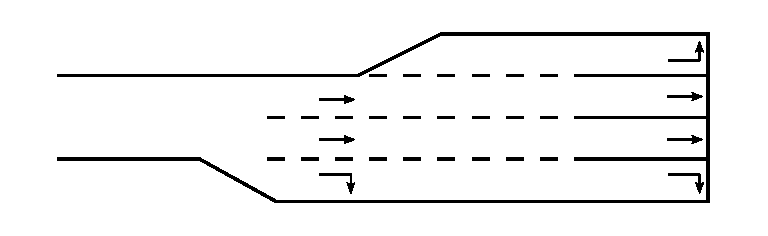
\includegraphics[width=0.475\linewidth]{extending/figures/signalslanes/real_road_layout.pdf}}
	{\label{fig:real_road_layout}}
  \createsubfigure%
	{Single queue, spill-back is not captured correctly}%
	{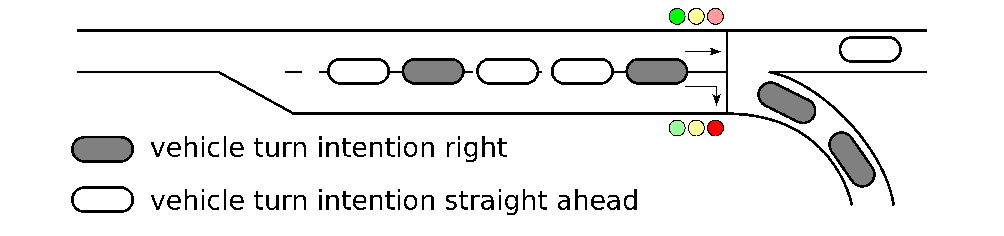
\includegraphics[width=0.48\textwidth]{extending/figures/signalslanes/single_queue_model_inkscape.pdf}}%
	{\label{fig:lanes_representation_single_queue}}%
}%
{info about source (optional)}

This section discusses the representation of transport networks with microscopically modeled traffic signals. 
In MATSim, the representation of  the transport network is a static, directed graph consisting of nodes and links. 
Links depict road segments while nodes can be interpreted as decision points in space that have a coordinate as attribute. 
The location of nodes in space is not supposed to vary over time. 
Nodes possess a geospatial interpretation and can be located in space. 
But, in contrast to links, nodes have no spatial dimension.  
The course of the road segments, however, is not specified and is inaccurate. 


Fig.~\ref{fig:real_road_layout} illustrates a typical layout of a real-world road segment with several turn pockets at its end. 
If the whole road segment is modeled as a single link with MATSim's queue model the first vehicle stopping at a red traffic signal at the end of this link will block all other approaching upstream vehicles, Fig.~\ref{fig:lanes_representation_single_queue}. 
In respect to the road layout shown in Fig.~\ref{fig:real_road_layout} this is not realistic. 
Fig.~\ref{fig:model_link_layout} sketches the layout for a more realistic modeling. 
Vehicles with distinct turn intentions do not block each other until the available space for queueing on the turn pocket is used completely, Fig.\ref{fig:lanes_representation_multiple_queue}. 

\createfigure%
{Caption in List of Figures}%
{Influence of traffic signals on traffic flow and spill-back can be modeled by a queue model, if the layout of turn pockets is considered.}
{\label{fig:lanes_representation}}%
{%
  \createsubfigure%
	{Part of the graph required to model the road layout}
	{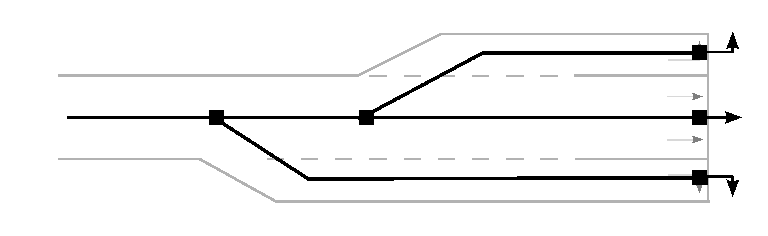
\includegraphics[width=0.475\textwidth]{extending/figures/signalslanes/link_lanes_layout}}
	{\label{fig:model_link_layout}}
  \createsubfigure%
	{Multiple queues, spill-back is captured correctly}%
	{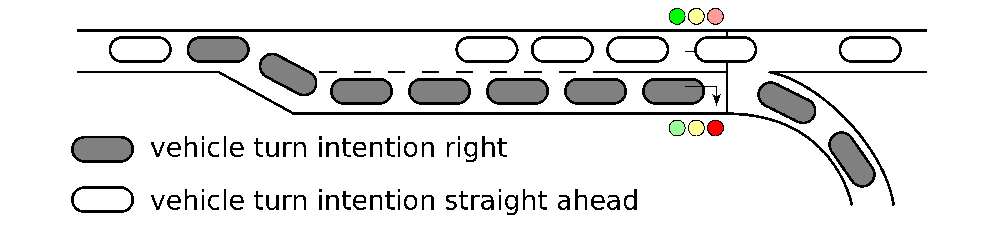
\includegraphics[width=0.48\textwidth]{extending/figures/signalslanes/multiple_queue_model_inkscape.pdf}}%
	{\label{fig:lanes_representation_multiple_queue}}%
}%
{info about source (optional)}

In principle you can model each turn pocket as single link, place traffic signals at the end of the link and you are done. 
But, considering overall project constraints, this has several implications for network modeling and routing. 

\mnote{motivation lanes}
In MATSim, all attributes relevant for the domain that differ from geospatial location are attached to links. 
If, e.g., speed limits or the number of lanes are attached as attributes to links, a node can also represent a point in space where one of these attributes changes.  

Many different attributes may be attached to the links of a transport network, e.g., traffic count data, transit stops, transit lines, speed limits, etc. 
Geospatial location may not be sufficient to describe the matching between attributes and links. 
Often, certain attributes are matched manually. 
If, for the representation of turn pockets, the network layout is changed, the manual matching must be repeated. 
This can result in huge effort. 
Further, a comparison between a simulation with and without an implicit model for turn pockets is difficult. 
Simulation models deliver different results for different network resolutions~\citep[][p.~38]{GawronPhd}.  
For comparison, one needs some algorithmic that traces the changes in network structure.  
If the network is changed to capture turn pockets, the shortest path algorithm is responsible to select the appropriate turn pocket on a route. 
If many turn pockets lead to the same downstream link, the number of required iterations is increased. 

\mnote{solution lanes}
To resolve this problem, the implementation in MATSim allows the modeling of a subgraph on top of a link that reflects the structure shown in Fig.~\ref{fig:model_link_layout}. 
Edges of the subgraph are called \alert{lanes}. 
Traffic flow on each lane is simulated nearly the same way as for links in the extended queue model. 
Just the calculation of minimum travel time slightly differs to avoid systematic errors of temporal resolution~\citep[][p.~38]{GawronPhd}. 
The calculation for lanes is set up in a way that is compatible to a link of the extended queue model without lanes, i.e., in freeflow conditions both models result in exactly the same travel times. 
This avoids further propagation of systematic errors. 
At the beginning of the link only one lane may exist. 
%
The next lane is determined by the necessity to be in the correct turning lane for the next downstream link of the vehicle's precomputed route.
According to the Cremer and Landenfeld approach, the vehicle is placed on the lane that currently contains the smallest number of other vehicles if there are several lanes leading to the same downstream link.
Note, that the lanes of the model have no 1:1 relation to the lanes existing on a link in reality.
The use of lanes implies a specification of the downstream links, thus, specific turning moves can be forbidden. 
This requires a modified routing of vehicles.

\subsection{Routing}

\mnote{Routing}
Within the overall simulation process introduced in Chapter~\ref{sec:matsim-overview} the use of lanes affects the routing module. 
Routes are specified within MATSim as sequence of links\footnote{In older version of MATSim, this can also be specified by a sequence of nodes.}.  
The shortest path algorithm is set up on link travel times. 
These do not reflect the travel time differences for turning moves modeled by the subgraph. 
In addition, turn restrictions cannot be captured by standard shortest path algorithms. 
To avoid these problems, the shortest path algorithm can be set up on the line graph. 
Thereby, the turn restrictions are considered when the line graph is created. 
The dynamic link travel times for the line graph reflect the link travel time on the original network plus the travel time for the specific turning move. 
Then, the shortest path calculation captures the effects of lanes without further modification. 

\mnote{Lanes \& Routing}
Within the overall simulation process introduced in Chapter~\ref{sec:matsim-overview} the use of lanes affects the routing module. 
Routes are specified within MATSim as sequence of links\footnote{In older version of MATSim, this can also be specified by a sequence of nodes.}.  
The shortest path algorithm is set up on link travel times. 
These do not reflect the travel time differences for turning moves modeled by the subgraph. 
In addition, turn restrictions cannot be captured by standard shortest path algorithms. 
To avoid these problems, the shortest path algorithm can be set up on the line graph. 
Thereby, the turn restrictions are considered when the line graph is created. 
The dynamic link travel times for the line graph reflect the link travel time on the original network plus the travel time for the specific turning move. 
Then, the shortest path calculation captures the effects of lanes without further modification. 


\begin{itemize}
	\item traffic flow linear to green time, see also LaemmerPhd
	\item Routing
\end{itemize}

\subsection{Findings}

\begin{itemize}
	\item Can you modify your network?
	\item Do you want to have a comparison between network with and without lanes?
\end{itemize}




\section{Iterations \& Learning}
\label{sec:signals_iterations_learning}


%\mnote{Equilibrium?}
Using Wardrop equilibrium assumptions and continuous link costs,~\citet{Smith1979ExistenceUniquenessStabilityEquilibria} shows the existence of a unique and stable static traffic equilibrium. 
This provides the underlying theory to prove, that traffic signal control influences route choice~\citep{Smith1979TrafficControlRouteChoice}. 
The existence of a dynamic traffic equilibrium is studied by~\citet{Smith1993ModelDynamicUE}. 
\citet{SmithVanVuren1993TrafficEquilibriumResponsiveControl} propose an optimization algorithm for dynamic assignments that takes traffic-responsive signal control into account.  
The dynamic formulations do not consider the physical extent of queues, they are built up on point-queues. 

%\mnote{Combined Problem}
The combined modeling of the traffic signal control and traffic assignment is subject of several other research lines. 
\citet{Meneguzzer1997ModelReviewTrafficAssignmentSignalControl} reviews their initial roots and defines the {\bf combined traffic assignment and control problem} (CTAC) as finding a tuple $(f^{*}, g^{*})$ of traffic flows $f$ and signal settings $g$ under policy $P$ that fulfills  
\[
f^{*} = f^{e}[g^{P}(f^{*})] \mbox{  or  equivalently } g^{*} = g^{P}[f^{e}(g^{*})]
\]
where $f^{e}$ is a function mapping signal settings to equilibrium traffic flows and $g^{P}$ a function mapping from traffic flows to signal settings under policy $P$.  
Nicely, the formulation shows the mutual interaction of traffic patterns and signal settings. 
A similar problem formulation is given by~\citet{CascettaGalloMontella2006SignalsWithStochAssignment}, studying the difference between global and local signal optimization. 
The time horizon, on that these interactions take place, is not captured by the formulations. 

%\mnote{Game theory}
Solution techniques for game theoretical models and mathematical programs with equilibrium constraints are similar, especially for bi-level, Stackelberg games~\citep{Hollander2006NonCooperativeGamesTransport}. 
Game theory provides techniques and terminology to describe the social dilemma of self-interest vs cooperation between distinct players. 
For transportation systems game theory provides ''a framework for modeling interactions between groups of decision makers when individual actions jointly determine the outcome''\citep{Fisk1984GameTheoryTransportationSystems}. 
The definition of a ``leader'' is required to model the decisions of a transport authority and the response of traffic participants as Stackelberg game. 
%
Mathematical programs also comprise such assumptions but they often are intrinsic to the model and not discussed. 
%
A broad review of games used to model and analyze transport systems was undertaken by~\citet{Hollander2006NonCooperativeGamesTransport}. 
Classical game theory is static an explicit representation of time is missing. 
In most cases traffic flows are modeled statically. 

%\mnote{Space \& Time}
Under the assumption that interactions between travelers and traffic signals over space and time have nicely behaved mathematical properties~\citet{Hu1997D2DFlowEvolutionReactiveSignalsDynasmart} use DYNASMART\footnote{see~\url{http://mctrans.ce.ufl.edu/featured/dynasmart/}, last access 17.05.2013} for simulation. 
Traffic signal control and travelers' reactions are studied in a day-to-day and real-time context. 
Traffic-responsive control may improve throughput of a traffic network. 
The peak load of the network stays equal. 
The travelers use the improvements to reduce schedule delay~\citep{Hu1997D2DFlowEvolutionReactiveSignalsDynasmart}. 
\citet{Burghout2007HybridSimulationAdaptiveSignal} build a hybrid simulation by a combination of a microscopic and a mesoscopic traffic simulation model. 
The replacement of a fixed-time control by a traffic-actuated signal control at two junctions changes the travel patterns in the city-wide network. 

%\mnote{Dynamics \& Game Theory}
Game-theoretic formulations for the dynamic interactions between traffic control and traffic assignment are given by~\citet{ChenBenAkiva1998GameDynamicTrafficControl}. 
Depending on the type of game used to model the problem, the quality of the solution with respect to the objective function differs.  
The solution of a monopoly game represents the optimal solution that can be used as benchmark. 
A Stackelberg equilibrium is superior to the Cournot-Nash equilibrium as user reactions are anticipated~\citep{ChenBenAkiva1998GameDynamicTrafficControl}\footnote{
%
The Cournot-Nash equilibrium is defined as follows: 
``In a noncooperative game between a traffic authority and highway
users, a combination of strategies $(g^*, h^*)$ is a Cournot(-Nash) equilibrium
$\Leftrightarrow$ control plan $g^*$ is the traffic authority's best
response to flow $h^*$, and flow $h^*$ is the users' 
%\kai{paper sagt user's (sing.), aber m.E.\ sollte es users' (plural) sein??} 
best response to control plan $g^*$'' \citep[from][]{ChenBenAkiva1998GameDynamicTrafficControl}.
%
\\
%
The Stackelberg equilibrium improves over the Cournot equilibrium in
that the traffic control authority anticipates the users' reactions:
``$\ldots$, a strategy combination $(g^*,h^*)$ is a Stackelberg
equilibrium $\Leftrightarrow$ it solves the following bilevel
programming problem: $\min_g Z[g,h^*(g)]$ such that flow $h^*(g)$ is
the users' best response'', where $Z$ is the traffic authority's
objective function \citep[after][]{ChenBenAkiva1998GameDynamicTrafficControl}.
%
\\
%
In the system optimum ($=$ monopoly game), the traffic authority also
controls the user flows; the optimization problem becomes: $\min_{g,h}
Z[g,h]$.
%
}.

Mutual effects between road users and two different road authorities responsible for traffic signal control are investigate by~\citet{VanZuylenTaale2004UrbanRingRoads} in an analytic, static setup, and by simulation.  
In a Stackelberg game, one of the road authorities takes the role of the leader. 
The other authority and the road users react to the decisions of the leader. 
Results for the analytical solution differ according to the leader of the Stackelberg game.  
Same holds for the presented dynamic simulation studies. 
Best results, however, are reported when both authorities cooperate and anticipate the road users' reaction on the traffic signal control. 
%\mnote{Physical Queues}
Noteworthy, the simulation model takes into account physical queue length~\citep{TaaleVanZuylen2003AnticipatoryTrafficControl} and is refined in further works to capture spill-back effects between links of the transport network~\citep{Taale2008Phd}. 
In a more general context, the importance of modeling physical queues for dynamic assignment is emphasized by~\citet{DaganzoAssign-w-queues}.  
The temporary limited effect of queue spill-back in conjunction with a dynamic assignment may lead to situations where the equilibrium is no longer unique.  

%\tododg{look at : I think so, should check the other Cascetta references in there? s.o. bzw discussion }

%\mnote{Agents \& Evolutionary Games}
In general, agent- and mechanism-design both can benefit from use of game theory~\citep[][pp.~666]{RusselNorvig2010ArtificialIntelligence}. 
Most mentioned approaches use classical game theory and the Nash equilibrium assumptions, i.e., the impact of a strategy is assumed to be fully known by all players. 
The approaches modeling interactions between traffic control and travelers that take time-scales into account use iterative solution techniques. 
Traffic assignment is solved iteratively and at least partly via simulation. 
\citet{Hu1997D2DFlowEvolutionReactiveSignalsDynasmart} report amongst other as result the number of ``days''~\footnote{one iteration represents one day} until convergence as measure of effectiveness. 
To describe the dynamic interactions between players, also evolutionary game theory can be used~\citep[e.g.~][]{HofbSigmBook}. 
While classical game theory looks for equilibrium solutions, evolutionary game theory searches strategies that are evolutionarily stable \citep[p.~348]{Bazzan2009ReinforcementLearningPrint}. 
Thus, use of evolutionary game theory helps when learning processes are included in the model. 
E.g., the agents that learn to control signalized junctions proposed in~\citet{Bazzan2005signalAgents} are useful if they are able to learn quickly but useless if learning takes infinite time. 
Evolution seems plausible on both sides of the game -- \citet[e.g.~][]{BazzanEtc2008co-evolution-of-tr-lights-lncs} signalized junctions \emph{and} car drivers are modeled as learning agents. 

\begin{itemize}
	\item Who is learning what? 
	\item No best way found
	\item Document what you have done
\end{itemize}


\section{Traffic Signals in MATSim}
\label{sec:signals_evaluation_conclusion}

\begin{itemize}
	\item Evaluation criteria manifold
	\item BUT: Matsim model only simulates a part of it
	\item Do Not over-interpret results, implement and interpret everything in respect to other simulation steps, document what you have done
\end{itemize}


\subsection{Conclusion, why -- again}

\begin{itemize}
	\item How to adapt the config file?
	\item Which additional files are needed?
	\item Refer to the user guide.
\end{itemize}

\begin{itemize}
	\item After reading a lot of constraints, why do not use another tool?
	\item Network wide effects
	\item Simulation results consistent with model's implementation 
	\item Economic evaluation
	\item Diversity 
	\item Go!
\end{itemize}

\section{Automatically Generated Module Information}
\label{sec:signals_config}
Module in the config: 
\begin{itemize}
	\item \lstinline|signalsystems|
\end{itemize}

Package:
\begin{itemize}
	\item \lstinline|org.matsim.signalsystems|
\end{itemize}

http://matsim.org/node/732

Literature: \citet[][]{GretherEtAl_ABMTRANS_2012, Grether_PhDThesis_2014, Neumann_MastersThesis_2008}
Auch Miss Ou-Paper ansehen: Optimierung von Lichtsignalen

\citet[][p.?]{BalmerEtAl_ResRep_bdktzrh_2009}


Information about signal light timing are available for the city of Zurich  \citep{STAPOZH-DAV_unpub_gtZH_2008} (\ref{ptl:zhCity}). Modeling of traffic lights was implemented for the project \emph{Westumfahrung} trough reducing the available link capacity. However, the used \emph{mobsim} (DEQSim) is deprecated (see Section \ref{sec:deqsim}).

Research and implementation efforts are undertaken to include individual traffic lights in other \emph{mobsims} (see e.g., (\ref{tl:docu}) and \citet[][]{Neumann_MastersThesis_2008}).

% -------------------------------------------

Lanes:

The lanes package has been implemented in conjunction with signal systems. Lanes are enabled in the \lstinline|scenario| configuration file section. The lanes package (\lstinline| org.matsim.lanes|) provides readers, where the class \lstinline|ModelLane| serves as the interface between the lane functionality and the mobility simulation. The lane definitions file needs to be specified in the \lstinline|network| configuration file section.

% ##################################################################################################################
